\chapter{Neural Networks Can Compute Any Function}


This is a condensed write-up of Chapter~4 of Nielsen's book. The objective is 
to present the main ideas of a proof that neural networks can approximate 
any continuous function.

\section{Step Functions and Function Approximation}

There are two main observations in this ``proof.'' First, that a single 
sigmoid neuron can approximate a step function; and second, given 
any interval on the real line $[a, b]$, one can construct a 
fixed-sized network of sigmoid neurons that takes as input a real 
number~$x$ and outputs a $1$ if and only if $x \in (a, b)$. 

It is easy to show that if we want a single sigmoid neuron to step-up 
from $0$ to $1$ at a point~$s$ on the real line, then this can be 
achieved by selecting a high enough weight, say $w = 1000.0$, 
and bias of $b = - s \times w$. This is shown in 
Figure~\ref{fig:nn_step_functions}.
\begin{figure}[ht]
\begin{center}
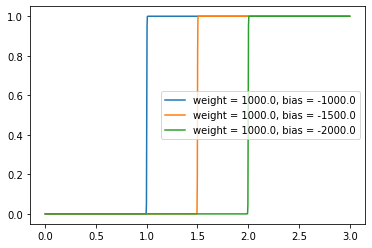
\includegraphics[scale=0.6]{stepfunctions.png}
\end{center}
\caption{Output of a single sigmoid neuron for different values of weight and bias}
\label{fig:nn_step_functions}
\end{figure}

We can now combine two sigmoid neurons which step up at points $s_1$ and $s_2$,
with $s_1 < s_2$, to create a network that outputs a $1$ if and only if $x \in
(s_1, s_2)$ as shown in Figure~\ref{fig:nn_rect_func}. The top neuron of the
hidden layer has a bias $b_1 = - s_1 \times w_1$, where $w_1$ is the weight of
the link between itself and the input node. We choose $w_1$ to be a large
enough number so that this neuron acts as a step function at the point $s_1$.
The bottom neuron in the hidden layer has bias $b_2 = - s_2 \times w_2$, where
$w_2$ is the weight of the link between itself and the input node. As before,
we choose $w_2$ to be large enough so that the bottom neuron steps up at $s_2$. 

Now the trick in making the output of the combined network to be a $1$ when the
input is in the interval $(s_1, s_2)$ is by adjusting the weights of the links
from the hidden layer to the output neuron. We set the weight of the upper link
from the top-most neuron to the output neuron to be $h$ and the weight of the
lower link to be $-h$. Here $h$ is just a very large number. The bias of the
output neuron is set to $-h/2$. The resulting output is then given by:
\[
    \sigma (h \cdot a_1 - h \cdot a_2 - h/2),
\]
where $a_1 = \sigma(w_1 x + b_1)$ and $a_2 = \sigma(w_2 x + b_2)$.
Now $a_1 = 1$ iff $x > s_1$ and $a_2 = 1$ iff $x > s_2$. Thus if $x < s_1$, 
the output is $\sigma(-h/2) \approx 0$; if $x \in (s_1, s_2)$, 
the output is $\sigma(h/2) \approx 1$; 
if $x > s_2$ the output $\sigma(-h/2) \approx 0$. 
At the boundary points, $s_1$ and $s_2$, 
the output is a number between $0$ and $1$. This is because the neurons 
can only approximate a step function. This construct forms the basis 
of how we can approximate arbitrary continuous functions from $\R^m \to \R^n$. 
\begin{figure}[ht]
\begin{center}
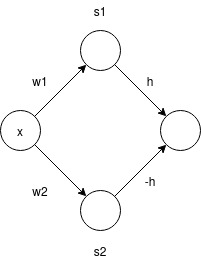
\includegraphics[scale=0.5]{RectFunction.jpg}
\end{center}
\caption{Network of sigmoid neurons to output a rectangle function.}
\label{fig:nn_rect_func}
\end{figure}
The output of such a network is shown in Figure~\ref{fig:x_step_function}. 
\begin{figure}[ht]
\begin{center}
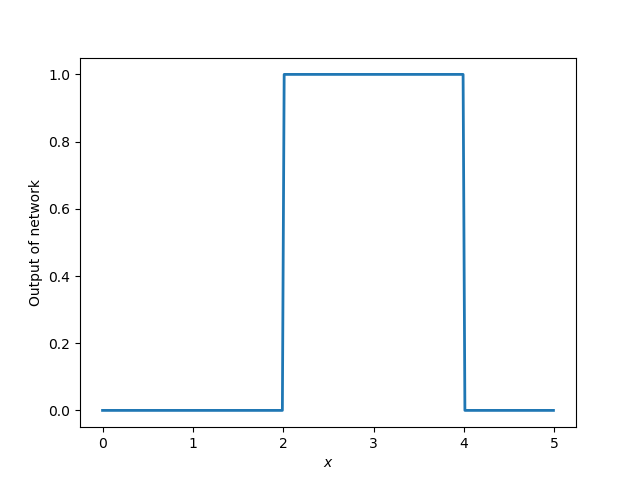
\includegraphics[scale=0.5]{xStepFunction.png}
\end{center}
\caption{Output of the network. $w_1 = w_2 = 10000.0$ and $h = 10000.0$}
\label{fig:x_step_function}
\end{figure}



\section{Functions of One Variable}

The network described in the last section acts as an indicator function
for an interval $[s_1, s_2]$ of the real line. Consider a function 
$f \colon \Rone \to \Rone$ whose mean value in the interval $[s_1, s_2]$ 
is $y$. If we were to now weight the output of the network by $y$ by 
adding an extra output node with a linear activation function, the resulting 
output of this new network will be a $y$ whenever $x \in (s_1, s_2)$ and a $0$ 
otherwise. Piecing together several of these networks would allow us 
to output the approximate value of $f$ over several intervals. 

In Figure~\ref{fig:one_variable_function}, we show a network that approximates 
a function $f$ over an interval $[s_1, s_5]$. In order to do this, this interval 
is first broken down into four sub-intervals $[s_1, s_2]$, $[s_2, s_3]$, $[s_3, s_4]$
and $[s_4, s_5]$. The top-most neuron from the second hidden layer from the left 
represents the output of the indicator function that detects whether the input $x$ 
lies in the interval $[s_1, s_2]$. This neuron is labelled $I[s_1, s_2]$ to 
represent this fact. The output weight from this neuron is labelled $f[s_1, s_2]$
which represents the average value of the function $f$ in the interval $[s_1, s_2]$.

The output neuron has a linear activation whereas the remaining neurons in the two 
hidden layers are sigmoid neurons. The network as a whole functions as follows: 
when $x \in [s_i, s_{i + 1}]$ for $i \in \{1, 2, 3, 4\}$, the corresponding sub-network 
$I[s_1, s_{i + 1}]$ outputs a $1$; all other sub-networks output $0$. The final output
of the network is then $f[s_i, s_{i + 1}]$, the approximate value of $f$ in this interval. 
By increasing the number of intervals, one can obtain better and better approximations 
of $f$ over larger intervals. This idea is used to generalize the result to 
functions of several variables. 

\begin{figure}[ht]
\begin{center}
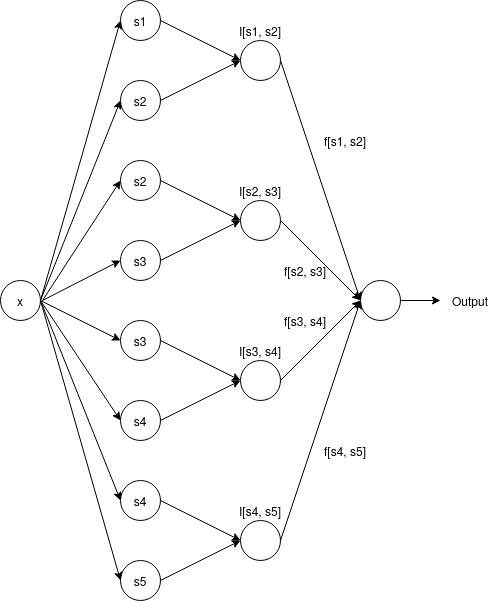
\includegraphics[scale=0.5]{OneVariableFunctions.jpg}
\end{center}
\caption{Network that approximates a function on the range $[s_1, s_5]$}
\label{fig:one_variable_function}
\end{figure}

We created a small program that approximates the function provided in 
Nielsen's book: $f(x) = 0.2 + 0.4 x^2 + 0.3 x \sin(15 x) + 0.05 \cos(50 x)$. 
We show some of the results in Figures~\ref{fig:one_variable_10neurons}.
\begin{figure}[ht]
\centering
\begin{minipage}[b]{0.4\textwidth}
\begin{center}
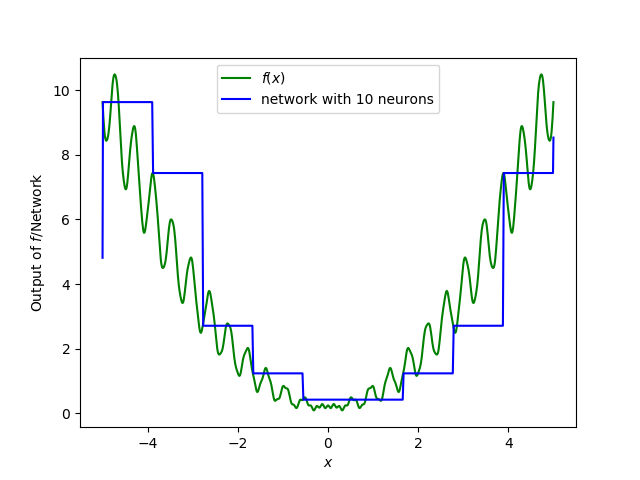
\includegraphics[width=\textwidth]{OneVar10Neurons.png} 
\end{center}
\end{minipage}
\hfill
\begin{minipage}[b]{0.4\textwidth}
\begin{center}
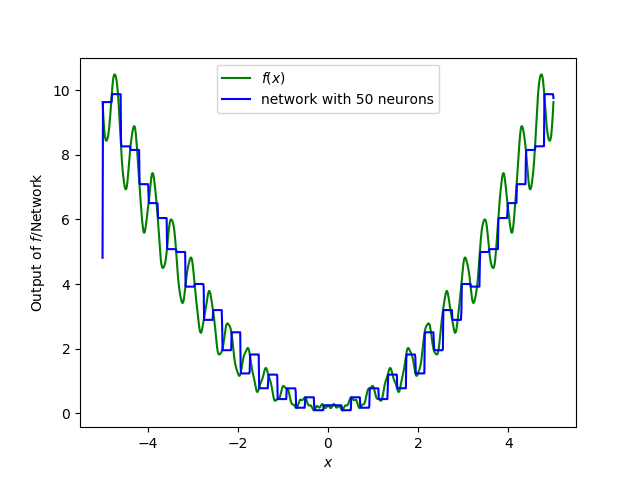
\includegraphics[width=\textwidth]{OneVar50Neurons.png} 
\end{center}
\end{minipage}
\caption{Approximating with 10 neurons and 50 neurons.}
\label{fig:one_variable_10neurons}
\end{figure}

\section{Functions of Several Variables}

In order to generalize this to functions of two variables, we need to first 
construct step functions on the plane. We could then construct networks 
that represent indicator functions for rectangular regions in $\R^2$. By taking a 
linear combination of such indicator functions with appropriate weights, we can 
approximate any continuous function $f \colon \R^2 \to \R^1$. 

The network used to approximate a step function in $\R^2$ is shown in 
Figure~\ref{fig:tower_function}. This network has two sub-networks: one 
for creating a step function along the $x$-axis and another for the $y$-axis. 
The construction of these sub-networks is exactly the same as in the case of 
one-variable functions with the difference being that the output neuron now has to 
output a $1$ iff $(x, y) \in (s_x^1, s_x^2) \times (s_y^1, s_y^2)$. This is achieved 
by adjusting the bias of the output neuron to $- 3h/2$, where $h$ is some large number.
  
Let us look at this network a little more closely. 
The top two neurons of the first hidden layer labelled $s_x^1$ and $s_x^2$ to indicate 
the fact that they help create the indicator function for the interval $(s_x^1, s_x^2)$ 
on the $x$-axis. Let their input weight and bias be $w_1, b_1$ and $w_2, b_2$, respectively. 
Similarly, the bottom two neurons of the first hidden layer and labelled $s_y^1$ and $s_y^2$.
Let their input weight and bias be $w_3, b_3$ and $w_4, b_4$, respectively. Now if the input 
to the network is $(x, y)$, the weighted input to the output neuron is given by:
\[
    h \cdot \sigma (w_1 x + b_1) - h \cdot \sigma (w_2 x + b_2) + h \cdot \sigma (w_3 y + b_3) 
    -h \cdot \sigma (w_4 y + b_4).
\]
The crucial observation here is that when $x \in (s_x^1, s_x^2)$ and $y \in (s_y^1, s_y^2)$ 
then this weighted input is $\approx 2h$; otherwise, this is $< h$. Hence the output in the 
first case is $\sigma (2h - 3h/2) = \sigma (h / 2) \approx 1$, whereas in the second case
is $\sigma (h - 3h/2) = \sigma (-h/2) \approx 0$. This holds whenever $h$ is some very large number.
The bias can be any negative number whose absolute value is between $h$ and $2h$. 
We just chose $-3h/2$.

Also note that we can extend this naturally for functions of three or more variables. For three 
variables, we would have another sub-network that creates an indicator for an interval 
$(s_z^1, s_z^2)$ on the $z$-axis. This sub-network would then be wired to the output neuron whose
bias would have to be modified to $-5h/2$. Again the bias can be any number whose absolute value 
is between $2h$ and $3h$. For an $m$-variable function, we will have $m$ sub-networks, each 
creating an indicator function for an interval along the appropriate axis, connected 
to the output neuron with bias $- (h + h - 1)/2 = - (2h - 1) / 2$. These can then be connected 
with other sub-networks for an extended range of intervals to approximate a function on this
range of intervals.     
\begin{figure}[ht]
\begin{center}
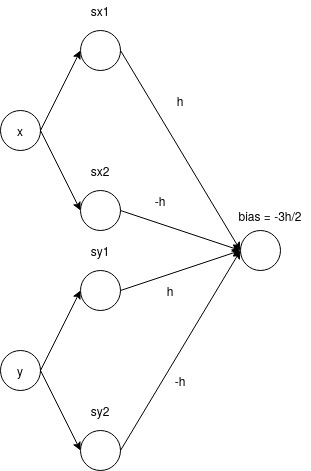
\includegraphics[scale=0.5]{TowerFunction.jpg}
\end{center}
\caption{Network that approximates a tower function in two variables}
\label{fig:tower_function}
\end{figure}

Finally, we consider the case of functions~$f$ from $\R^m$ to $\R^n$. Any such function can be 
decomposed into $n$ functions $f_1(x_1, \ldots, x_m), \ldots, f_n(x_1, \ldots, x_m)$ 
from $\R^m \to \R^1$. Hence this case can be handled by combining 
$n$ networks one for each of the $n$ functions.  



